\documentclass{article}
\usepackage[utf8]{inputenc}
\usepackage{graphicx}

\title{Gov 1790 Final Exam Review}
\author{Jack Deschler}

\begin{document}

\maketitle

\section*{C. Unipolarity and its Discontents}
\subsection*{Hegemony and Empire}
\textbf{Kindleberger}: \textit{Dominance and Leadership in the International Economy}\\
\renewcommand\labelitemii{$\cdot$}
\begin{itemize}
    \item leadership rejects exploitation
    \item leadership focuses on producing enough public goods
    \begin{itemize}
        \item even if against the follower's short term interests
    \end{itemize}
    \item leadership can degenerate into exploitation $\rightarrow$ ``power corrupts and absolute power corrupts absolutely"
    \item Was US post-WWII searching for domination? French said yes, US said no
    \item Leaders often are needed to ``assume the burden"
    \begin{itemize}
        \item Look at post-WWI with a leadership vaccuum
    \end{itemize}
    \item Leadership systems can collapse from within
    \begin{itemize}
        \item burdens get too high, payoffs too low
        \item too many free riders, seeking bigger and bigger free rides
    \end{itemize}
    \item \textbf{a hegemon is needed???}
    \begin{itemize}
        \item ``without a stabilizer, the world is unstable"
        \item ``a world of Denmarks is as unstable as a world of Prussias"
    \end{itemize}
\end{itemize}
\textit{Important points from reading guide}
\begin{enumerate}
    \item What does Kindleberger thing about American Hegemony? (I think he is in favor?)
    \item Pay attention to the public good framework
\end{enumerate}
\bigskip
\textbf{Nexon}: \textit{What's This, Then? ``Romanes Eunt Domus"?}
\begin{itemize}
    \item Is USA a \textit{unipolar power} or a \textit{hegemonic power} or an \textit{informal empire}
    \item Arguments \textit{for} empire
    \begin{itemize}
        \item US has WAY more military/economic capabilities than rivals
        \item breadth/depth of USA military basing in other states
        \item scope of American influence (incl. in IMF/World Bank)
        \item we have removed other governments from power
    \end{itemize}
    \item distinction only matters if it changes how we think about USA/what we do
    \item avoid ``empire box" fallacy $\rightarrow$ not all empires are the same
    \item Key difference btw Empire and Hegemony is that Empire has no connections between the spokes on the wheel\\
    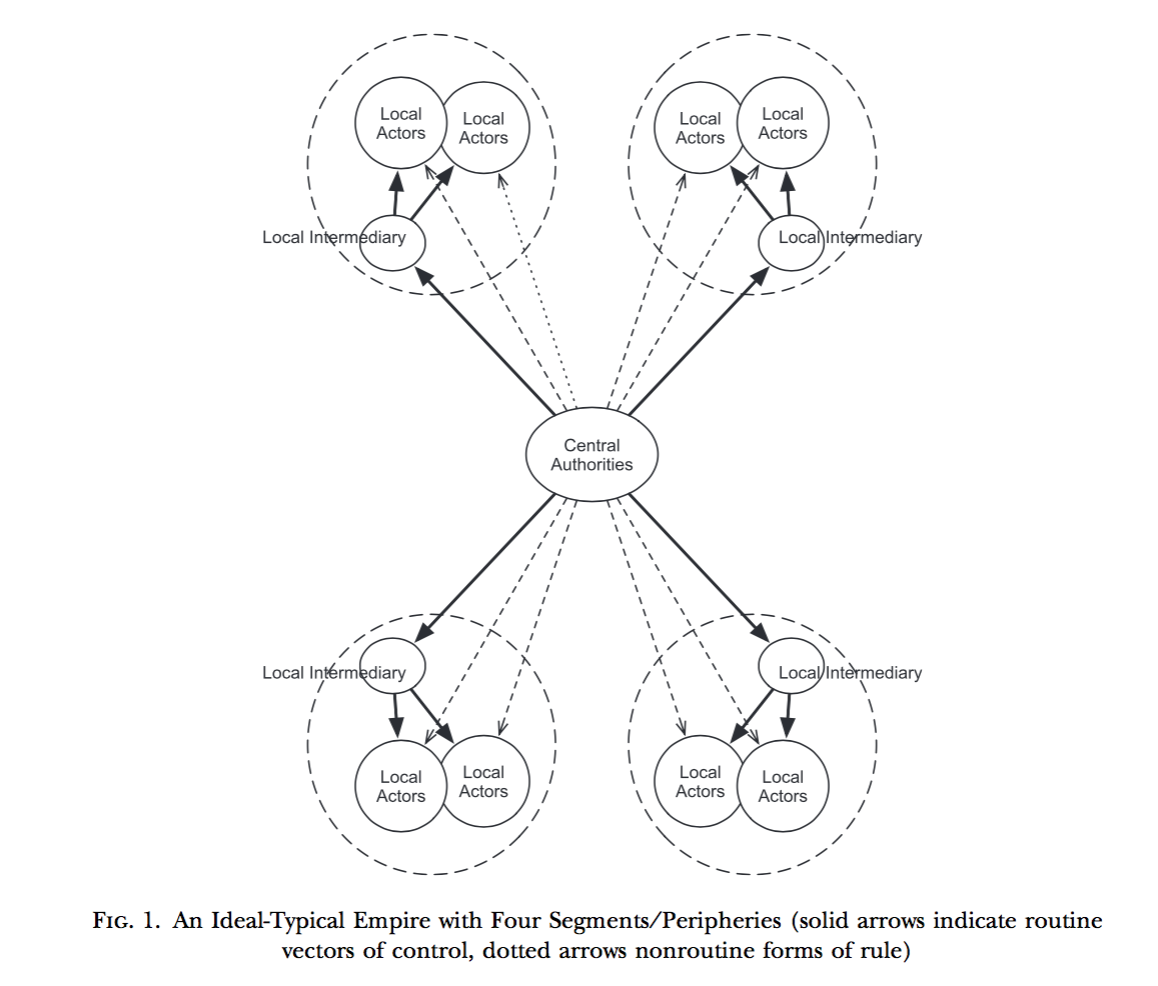
\includegraphics[width=\textwidth]{empire.png}
\end{itemize}
\textit{Important points from reading guide}
\begin{enumerate}
    \item Not normative
    \item Key is \textbf{Empire as an Ideal Type} section (see above image
    \item key terms will be principal-agent, cross pressures, etc.
\end{enumerate}
\subsection*{Anti-Americanism}
\textbf{Katzenstein and Keohane}: \textit{Varieties of Anti-Americanism: A Framework for Analysis}
\begin{itemize}
    \item Left (what we do) and Right (who we are) are both wrong about anti-americanism
    \item negative opinion can \textit{lead} to bias (AA), but does not necessarily indicate it
    \item AA: \textit{a psychological tendency to hold negative views of the United States and of American society in general} (note the word \textbf{tendency})
    \item opinion $\neq$ distrust $\neq$ bias
    \begin{itemize}
        \item \textit{opinion}: temporary, often the result of one specific policy, may not really influence policies
        \item \textit{distrust}: can change the willingness to work with USA, easily can become opposition
        \item \textit{bias}: people process information differently, very seriously affects policy
    \end{itemize}
    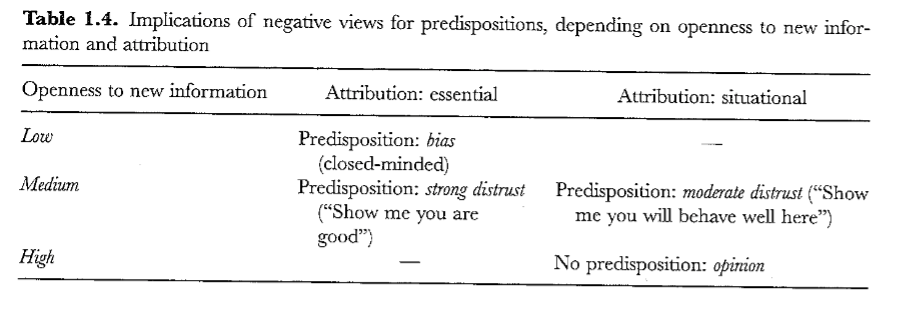
\includegraphics[width=\textwidth]{opdistbias.png}
    \item Can look at Tsunami Relief as an sort-of experiment (global diplomacy)
    \item \textbf{TYPOLOGY OF ANTI-AMERICANISM}
    \begin{enumerate}
        \item \textbf{Liberal AA}: USA criticized for not living up to its own liberal ideas, prevalent in developed societies (GB, France), feeds on hypocrisy
        \item \textbf{Social AA}: against the injustices in US policy (rich/poor imbalance), reliance on market conditions, there are genuine value conflicts (often from other types of democracies)
        \item \textbf{Sovereign Nationalist AA}: focused on control of their own politics, and their national identities. USA often at odds with this. Sovereignty used as a shield against USA. This tends to play well in domestic politics. See China. 
        \item \textbf{Radical AA}: hostility to America's core identity, and belief that USA stands in opposition to moral values. See USSR, and more recently, North Korea, Cuba. Cannot be combated, unless we change our political and economic systems. Argues for eventual destruction of USA. Not good.
    \end{enumerate}
\end{itemize}
\textit{Important points from reading guide}
\begin{enumerate}
    \item Definitions important
    \item Table 1.4 (above) on distrust vs. opinion vs. bias important
    \item TYPOLOGY very important
\end{enumerate}
\bigskip
\textbf{Datta}: \textit{The Decline of America's Soft Power in the United Nations}
\begin{itemize}
    \item \textbf{soft power} ability to attract others by legitimacy of US policies and the values that underlie them (notably not military/hard power)
    \item attitudes towards US matter when voting in the UN General Assembly $\rightarrow$ AA has consequences!
    \item though realists may say that the UN does not matter, the UN gives legitimacy to actions that it sanctions (legitimacy impt for the Hegemon)
    \item America is becoming less and less well-like in the world!!!!!
    \item Anti-Americanism may be correlated with Anti-Bushism $\rightarrow$ leaders matter!
    \item purse does not seem to matter much (foreign aid), and having an alliance only matters sometimes
    \item RESULTS: AA predicts a decline in soft power (THIS IS BAD)
    \item idea: democracies are more attuned to public opinion (and thus AA) than other countries
\end{itemize}
\textit{Important points from reading guide}
\begin{enumerate}
    \item what are the results?
    \item what is soft power?
    \item how does he measure AA?
    \item implications for Trump era?
\end{enumerate}

\subsection*{The Rise of China}
\textbf{Friedberg}: \textit{The Future of U.S.-China Relations: Is Conflict Invevitable?}
\begin{itemize}
    \item Six points of view on future of relations with China
    \begin{itemize}
        \item \textit{Liberal Optimists}: economic exchanges will create good will and incentives to avoid conflict, international institutions and democratization will help
        \item \textit{Realist Pessimists}: the hegemonic war is coming, China's power is rising, aims expanding, US is in the way (also idea that the ``century of humiliation" will make China more aggressive)
        \item \textit{Realist Optimists}: China's power is not increasing as quickly as we think, US is very far ahead, no war! China's aims are not as expansive as we think, etc.
        \item \textit{Liberal Pessimists}: as China democratizes, it will become volatile, and bad things will happen, ``hypernationalist rhetoric" is increasing. Additionally, the US may be on the crusade, esp. as China democratizes. 
        \item \textit{Constructivist Optimists}: Increasing participation by China in international institutions will lead them to adopt the global norms, which will shift their ideas of their nation, so no war! Culture change will keep us safe!
        \item \textit{Constructivist Pessimists}: China will see US as an ``intrusive bully" and not like what we do
    \end{itemize}
    \item All are plausible, we likely end up somewhere in the middle, when forces balance out. People disagree as to how
    \begin{itemize}
        \item \textit{Simple preponderance}: some forces simply outweigh all the other forces (liberal optimists and realist pessimists would argue this)
        \item \textit{Additive effects}: similarly aligned forces will combine to push us to conflict or peace (like institutions and the assymetric power balance). We will then act in ways that confirm our beliefs.
        \item \textit{Offsetting effects}: everything cancels the other side out, and we end up at the uneasy place of today for a while
    \end{itemize}
\end{itemize}
\textit{Important points from reading guide}
\begin{enumerate}
    \item Focus on six explanations, which you find most convincing
    \item also on three mechanisms of analysis
    \item overall conclusion: I think its that institutions will help us to peace
\end{enumerate}
\bigskip
\textbf{Nathan and Scobell}: \textit{How China Sees America: The Sum of Beijin's Fears}
\begin{itemize}
    \item China is a ``great power"
    \item China fears that the US is a ``revisionist power", bent on subjecting China to its values
    \item USA is omnipresent for China's security concerns (four rings), and China cares more about the negative policies than the positive ones
    \item China believes that US wants to maintain hegemony, so as China rises, US will resist that rise
    \item US has significant economic and military power
    \item China thinks US goal is to spread democracy
    \item hard to read US policy intentions bc of POTUS vs. Congress, and the two different parties
    \item Obama: ``strategic reassurance"
    \item Idea: US will remain the Hegemon, but world order should make a larger place for China
    \item BUT US should maintain military dominance, and ensure that global legal systems ramin in favor of the West
\end{itemize}
\medskip
\textbf{Gray and Navarro}: \textit{Donald Trump's Peace Through Strength Vision for the Asia-Pacific}
\begin{itemize}
    \item US military pivot to Asia-Pacific under Obama was a failure
    \item Especially since Obama cut the military, the pivot seemed BS
    \item Obama billed TPP as a security measure against China
    \item US losing sway with strategic allies in AP
    \item Trump: no more ``bad" trade deals (like TPP), pursue peace through strength (military muscle flexing?)
    \item also Trump: SK and Japan must step up their fair share of the military burden in AP
\end{itemize}
\textit{Important points from reading guide}
\begin{enumerate}
    \item there is a DEBATE between Nathan/Scobell and Gray/Navarro. Make sure you understand the DEBATE
    \item Nathan/Scobell: we need military power, but also a host of other things, like working with allies, trade deals, higher education back home (to educate Chinese students), regain legitimacy
    \item Gray/Navarro: MILITARY POWER MILITARY POWER NO BAD TRADE DEALS
    \item me: Nathan and Scobel I think
\end{enumerate}
\bigskip
\textbf{Nye and Wang}: \textit{The Rise of China's Soft Power and Its Implications for the United States}
\begin{itemize}
    \item China's soft power comes from its cultural relevance in world affairs, as well as its policies. That said, it still does not have the cultural influence of the USA (things like Hollywood, American sports)
    \item China has increased its diplomacy recently, which has increased its regional soft power
    \item China may be limited by its need to also build up its military, and its less than ideal domestic politics situation, also the brain drain
    \item US and Chinese soft power is sometimes in conflict, sometimes in concert (this makes intuitive sense)
    \item Americans do not like China as a cultural symbol, and vice versa (sorta, they want ``multipolarity")
    \item NOT a zero sum game
    \item it makes sense for China to build up soft power, as the USA far outstrips literally everyone in hard power
\end{itemize}
\textit{Important points from reading guide}
\begin{enumerate}
    \item Make sure you can answer:
    \begin{enumerate}
        \item where does China's soft power come from?
        \item what may limit it?
        \item is it a zero sum game w/ US soft power?
    \end{enumerate}
    \item They argue that the Chinese pursuit of soft power makes sense given a ``sophisticated realist strategy", and it does, but Mearsheimer, Waltz, and co. would disagree because SOFT POWER MEANS NOTHING TO REALISTS
\end{enumerate}
\section*{D. The Logics of Political Violence}
\subsection*{Terrorism}
\textbf{Mueller}: \textit{Six Rather Unusual Propositions About Terrorism}
\begin{itemize}
    \item Six Propositions
    \begin{enumerate}
        \item Terrorism has limited direct affects
        \item The true costs of terrorism come from the fear and overreaction to an attack
        \item Terrorism industry is a major part of the terrorism problem (think media, politicians, ``risk entrepeneurs")
        \item Policies about terrorism should focus on reducint fear and overreaction rather than actually reducing the limited direct effects of terrorism
        \item Doing nothing after a terrorist attack is not necessarily a bad idea
        \item Despite US overreaction, the war on terror (he says campaign against terror) is going well $\rightarrow$ home states have incentive to cooperate with international threats
    \end{enumerate}
\end{itemize}
\textit{Important notes from reading guide}
\begin{enumerate}
    \item know the six propositions
    \item think about if you agree
\end{enumerate}
\bigskip
\textbf{Pape}: \textit{The Strategic Logic of Suicide Terrorism} 
\begin{itemize}
    \item traditional studies simply treat suicide attacks as just one tactic, so are unable to explain its rise
    \item religions fanatacism does not adequately explain the rise either, many suicide attacks come from Marxist groups
    \item IDEA: suicide terrorism follows a stategic logic: five principles
    \begin{enumerate}
        \item it is \textit{strategic}, and is part of a larger campaign
        \item designed to make modern democracies (like USA) make concessions towards national self-determination
        \item it has become more common because it works in achieving these goals
        \item moderate campaigns are more likely to achieve their goals than more ambitious ones, as moderate concessions are more likely to be made
        \item best way to combat is to reduce confidence that the attacks will work
    \end{enumerate}
    \item key goal of suicide terrorism is to COMPEL a policy change from a target govt, by inflicting damage on the opposing society
    \item the suicide part magnifies the coercive affects by:
    \begin{enumerate}
        \item making it much more likely the mission succeeds, as the attacker is expecting to die
        \item signalling the likelihood of more attacks to come (the art of martyrdom)
        \item deliberately violating norms, so they increase the stakes, and make future attacks more credible
    \end{enumerate}
    \item suicide terror is high cost, so makes sense when there are high stakes (typically occupation of a homeland), and as a last resort
    \item democracies likely to be the target because they respond to public opinion
    \item because of asymmetry, the attacked state always has more power, and can thus punish in kind
    \item suicide terrorism doesn't work all the time, but it works better than other kinds (about half the time in the study)
    \item that said, it is unlikely to achieve ambitious goals: it does not change interests in the issues at stake, and so it cannot do \textit{too} much
    \item POLICY LESSONS: offensive military actions/concessions will not work (unless obv we concede the big goal), so we must make it very, very hard to achieve the goals, and undermine the effectiveness
\end{itemize}
\textit{Important points from the reading guide}
\begin{enumerate}
    \item Terrorists ARE NOT irrational fanatics
    \item Suicide bombing has become more popular because it works
    \item tests method by looking at suicide bombing campaigns, and whether or not they achieved their goals
    \item skip case study on Hamas/Israel if you understand his argument (cite in a paper tho?)
\end{enumerate}
\bigskip
\textbf{Abrahms}: \textit{What Terrorists Really Want: Terrorist Motives and Counterterrorism Strategy}
\begin{itemize}
    \item Strategic model is CONTRADICTED by 7 common tendencies of terrorists THE SEVEN PUZZLES
    \item The Strategic Model (Pape) rests on three key assumptions
    \begin{enumerate}
        \item terrorists are motivated by stable/consistent political goals, which are encoded in their political platforms
        \item terrorism is a ``calculated course of action", and is measured by efficacy, more specifically, terrorists resort to terrorism when political avenues are blocked
        \item decision to use terrorism is based on the ``logic of consequence", and its effectiveness is weighted against other options
    \end{enumerate}
    \item \textbf{The Seven Puzzles}
    \begin{enumerate}
        \item terrorism is ineffective at coercing governments
        \item terrorism is often the first resort, not the last one
        \item terrorists do not compromise (we would expect this if they were rational actors)
        \item ``protean" political platforms, as their platforms change frequently (ex: Action Directe moving from Israel to nuclear energy to the Church)
        \item anonymous attacks, these would not be expected if terrorists were trying to further political goals
        \item terrorist fratricide (ex: Tamil Tigers), many times they fight each other instead of their common enemy
        \item never-ending terrorism, even when it isn't working (look at assumption 3 of strategic model)
    \end{enumerate}
    \item Instead, what they really want is social solidarity (the natural systems model)
    \item Natural Systems Model: there is often a disconnect between the official goals of an organizations and the goals of its members, members are searching for the social benefits of being part of an organization
    \item Unmarried young men, looking for brotherhood, social solidarity join terrorist organizations (finding: key scope condition is knowing someone else who joined)
    \item We can see this because many foot soldiers never understand their organization's political goals (which we would not expect with the strategic actor model)
    \item The Natural Systems model solves the puzzles (think about it!)
    \item Implications for policy: concessions and stuff mean literally nothing, must instead break the bonds of brotherhood, use social network analysis, drive a WEDGE, and then make sure people are not alienated from everyday society
\end{itemize}
\textit{Important notes from reading guide}
\begin{enumerate}
    \item direct CRITICISM of Pape (a DEBATE perhaps?)
    \item make sure you understand the strategic model, and why the seven puzzles challenge it
    \item ensure that you understand the Natural Systems (solidarity seeking model) and pick the one you like better
    \item almost like this is a DEBATE
\end{enumerate}
\bigskip
\textbf{Kydd and Walter}: \textit{The Strategies of Terrorism}
\begin{itemize}
    \item Must understand strategies in order to craft counterstrategies
    \item core of argument: terrorist violence is a form of costly signaling, and they seek to alter the audience's beliefs about terrorist abilities
    \item 5 strategies: attrition, intimidation, provocation, spoiling, outbidding
    \item Definition: terrorism is the use of violence against civilians by nonstate actors to attain political goals
    \item typical goals: regime change, territorial change, policy change, social control, status quo maintenance
    \item uncertainty (about trustworthiness, power, resolve) causes conflict\\
    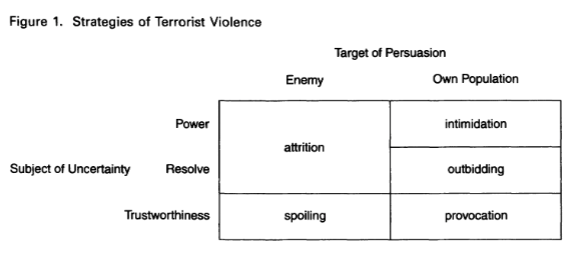
\includegraphics[width=\textwidth]{terroriststrats.png}
    \item Five Strategies
    \begin{enumerate}
        \item attrition: inflict (or have potential to) serious enough costs to cause enemy to submit to demands. Works better if you are hard to hit back (then you have attrition problems as well). Five counterstrategies:
        \begin{enumerate}
            \item concede nonessential issues in exchange for peace
            \item targeted retaliation, if you won't concede the issue
            \item harden defenses to minimize impacts
            \item deny access to most destructive weapons
            \item minimize psychological costs of terrorism (Mueller)
        \end{enumerate}
        \item intimidation: demonstrate that terrorists have the power to punish anyone who disobeys them. Best response is to retake territory in discrete chunks and decisively (clear and hold)
        \item provocation: get them to hit you back so that people become sympathetic in order to get the people on your side. Best response is to not inflict damage when you hit back, or to not hit back
        \item spoiling: sabotage the peace (Veto Players) between moderates and the government, leaving no hope for future peace
        \item outbidding: groups want to be zealots, not sellouts (see Hamas/Fatah)
    \end{enumerate}
\end{itemize}
\textit{Important notes from reading guide}
\begin{enumerate}
    \item focus on the taxonomy of goals, and the attached figure
\end{enumerate}
\subsection*{Counterinsurgency and Asymmetric Conflict}
\textbf{Kilcullen}: \textit{Countering Global Insurgency}
\begin{itemize}
    \item Terrorism is a strategy of the Global Jihad Counterinsurgency
    \item so it isn't ``War on Terror" but really ``War on the Global Islamic Counterinsurgency"
    \item There are active Islamist insurgencies practically everywhere, but especially in the historical Caliphate
    \item Theaters are linked, implying that it truly is global
    \item financial links, marriages, propaganda materials, etc. (note that Bin Laden was not a leader)
    \item similar techniques, doctrine and procedures (they found this on a CD apparently)
    \item thus the global jihad exists, but is a ``loosely aligned confederation of independent networks" not a unified group
    \item and the jihad itself is best understood as an \textit{insurgency}: a popular movement that seeks to overthrow the status quo through subversion, political activity, insurrection, armed conflict, and terrorism
    \item terrorism (using Kydd and Walter def.) is merely a tactic of the insurgency
    \item thus the war on terror should really be a massive COIN operation, and we should stop trying to fight terrorism, which is impossible (see Mueller)
    \item global insurgency is much harder to fight than a national level one, as coordination is significantly more difficult
    \item classic COIN: deny enemy sanctuaries, prevent entry to theater, isolate from support. All of these are harder for a global insurgency
    \item US strategy in War on Terror, seems to be ``aggregation" (lumping all terrorists together). With the global insurgency, we want ``disaggregation"
    \item if we can break apart the global jihad, COIN will work. We must break the links between different groups
    \item would mean that the war has three tiers: global, regional, local
    \item Disaggregation would focus on:
    \begin{itemize}
        \item attacking the web of dependency
        \item breaking links between theaters of operation
        \item denying linking between local and regional/global actors
        \item stopping information flows
        \item denying sanctuaries (COIN)
        \item isolating from local populations (COIN)
        \item disrupting inputs from the source to worldwide theaters
    \end{itemize}
    \item we also need some carrot to go along with the stick $\rightarrow$ the constitutional path
    \item key point: applying COIN to the global insurgency gives us \textit{disaggregation}
\end{itemize}
\medskip
\textbf{Porch}: \textit{The Dangerous Myths and Dubious Promise of COIN}
\begin{itemize}
    \item COIN DOES NOT WORK
    \item COIN has not worked historically, COIN projects Western values, etc.
    \item COIN itself is merely a small subset of tactics
    \item `hearts and minds' does not work! it does not create lasting stability
    \item old strategies for dealing with asymmetric insurgencies really don't work, so we got COIN during the People's War
    \item COIN proponents: we just misread Vietnam, COIN would have worked, there is a right and wrong way to fight insurgents, and COIN is the right way (hearts and minds)
    \item surprise, no one is particularly good at COIN, and it does not work
    \item population centric $\neq$ population friendly
    \item the times the Brits did it, they didn't even do hearts and minds, just did collective punishments
    \item Conclusion: COIN is not a separate category of warfare, COIN doesn't even work, we lost Vietnam for different reasons
\end{itemize}
\textit{Important notes from the reading guide}
\begin{enumerate}
    \item this is a DEBATE
    \item how does Kilcullen define insurgency? why is it different from terrorism?
    \item Kilcullen claims that the distinguishing feture of jihadists is not terrorist tactics, but their global scope
    \item How does Kilcullen say we should win the War on Terror?
    \item Porch: focus on what he says about how successful population-centric warfare is, and if it is applicable
\end{enumerate}
\subsection*{Civil Wars}
\textbf{Brown}: \textit{The Causes of Internal Conflict: An Overview}
\begin{itemize}
    \item long-simmering hatreds are not a good explanation of internal conflicts
    \item Four types of factors for permissive conditions\\
    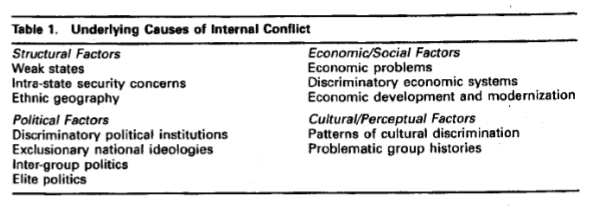
\includegraphics[width=\textwidth]{permissiveconditions.png}
    \item weak states can lead to security dilemmas with internal groups
    \item elite politics matter especially in times of turmoil
    \item but these are only the permissive conditions (important!)
    \item There must also be a proximate cause for the internal conflict\\
    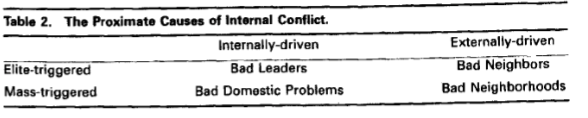
\includegraphics[width=\textwidth]{proximatecauses.png}
    \item domestic elites play a key role in the proximate causes
    \begin{enumerate}
        \item ideological conflicts
        \item criminal assaults on state sovereignty
        \item power struggles
    \end{enumerate}
    \item important point though, why do people follow the desperate domestic elites?
    \item two factors: antagonistic group histories and mounting economic problems
    \item Policy Implications
    \begin{enumerate}
        \item conflict prevention should be two-faced: fix underlying conditions (permissive conditions), and halt the proximate causes
        \item there are FOUR sets of proximate causes, watch out for all of them!
        \item focus on domestic elites, they can often spark the conflicts
    \end{enumerate}
    \item we are not as helpless as we may think
    \item there is not a single factor that is responsible for these things (like ancient hatreds)
\end{itemize}
\textit{Important notes from the Reading Guide}
\begin{enumerate}
    \item no real argument, just a summary
    \item underlying causes are different than proximate causes
    \item look at the tables (above)
    \item domestic elites less important
\end{enumerate}
\bigskip
\textbf{Lots of Authors}: \textit{Each with their own short article}
\begin{itemize}
    \item Fotini Christia: civil war scholarship says this won't end quickly, as there are lots of actors, and fragmented groups, too many veto players, and since outright military victory is hard, it probably won't end soon or well!
    \item Laia Balcells and Stathis Kalyvas: Syrian Civil War is a conventional war, not an irregular (guerrilla) war, so it could end quickly, as conventional civil wars tend to do
    \item James D. Fearon: there is really no hope for an agreement in Syria, as all the veto players will never be happy, the rebels have no reason to settle, neither does Assad, so we need third party intervention to supervise power sharing, but then the US won't be able to extricate itself, too much factionalism, etc.
    \item David E. Cunningham: lots of veto players in Syria, which will make the conflict resistant to resolution, as multi-party civil wars are quite difficult to resolve
    \item Barbara F. Walter: we know four things about how civil wars end:
    \begin{enumerate}
        \item they don't end quickly
        \item more factions, longer war
        \item most end in decisive military victories, not negotiated settlements
        \item the ones that end in negotiated settlements divide power based upon position on the battlefield, and minority position in govt makes you vulnerable to reprisals
    \end{enumerate}
    \begin{itemize}
        \item so no, Syria will not end quickly, and if it does it won't end well, or in negotiation
    \end{itemize}
    \item Alexander B. Downes: Even if we overthrow Assad, we will face opposition from the radical rebel factions, and spoilers form the less radical factions. This is bad. By endorsing overthrow, USA has contributed to deadlock. A new war would follow between rebel groups, and this would not end well. So if we want a negotiated end, Assad must stay in some form of power.
\end{itemize}
\section*{Arms control-alt-delete}
\subsection*{Nuclear Weapons}
\textbf{Waltz}: \textit{More May Be Better}
\begin{itemize}
    \item important to note that nuclear weapons \textit{have} proliferated vertically, as arsenals have grown
    \item Remember that international politics, according to realists, is an anarchic self-help system, in which states only want survival
    \item ``defense" (making it very hard to inflict damage), is very different than ``deterrence" (ensuring that you will hit them back super hard)
    \item second-strike nuclear forces are \textit{deterrent} forces
    \item strong deterrent forces make the risks of war much higher, and states will not run those risks for minor gains
    \item deterrence makes war less likely, especially nuclear deterrence, because there is less of a way to make a miscalculation about the oppositions strength (they have nukes, they are strong)
    \item hard for unstable countries to build nukes, because nukes take a long time to build
    \item contenders in an internal power struggle have no incentive to use nukes (what would they hit?)
    \item nukes also make you deal \textit{more cautiously} with your neighbors, as they can murder you (think USSR and China)
    \item if you have nukes, you can't act recklessly in world politics, because people will be scared of you and stop you
    \item can't assume you will remain anonymous if you fire a nuke, so no one will fire a nuke anonymously (cause the consequences will be high af)
    \item nuclear weapons also make poor offensive weapons (are you really gonna nuke territory you're trying to conquer @South Korea)
    \item fear of small powers building up nuclear forces is that they may prompt already nuclear power powers to strike, but they will not strike with nukes
    \item its also hard to find nukes to strike them, they can be moved and hidden easily
    \item and if we are afraid that terrorists would steal and hide a bomb, we have to be aware that states will also be able to hide the bomb well before the terrorists get it
    \item three requirements for a deterrent force:
    \begin{enumerate}
        \item part of the force must \textit{appear} to be able to survive and attack and be able to strike back (preclude preemption)
        \item must not require early firing (there may be false alarms)
        \item command and control must be maintained reliably
    \end{enumerate}
    \item note this means that small nuclear powers only need small arsenals
    \item to deter you only need to be able to inflict severe damage, not destroy like half a country (ex: will the US really risk San Francisco to North Korean nukes)
    \item two sides to deterrence: physical (can they build it), psychological (will the adversary believe the threat)
    \item think Hitler: would he really have attacked with nukes, or even in the face of nukes?
    \item but would Hitler have shot nukes once he lost? probs not: with inevitable defeat, no one would follow his orders, and \textit{no nuclear nation will be pressed to the point of a decisive defeat for this very reason!}
    \item RE arms races, they don't actually matter much once states have their small second-strike forces
    \item key point: nuclear weapons negate conventional military superiority
    \item US and USSR \textit{hated} each other, yet never actually fought a conventional war (NUKES)
    \item think about the NK logic! (@Narang's lecture)
    \item nukes probably kept the cold war cold
\end{itemize}
\textit{Important points form reading guide}
\begin{enumerate}
    \item Waltz is a BoP Realist who's opinions go against typical American policy
    \item think about if you agree with the broad argument he makes? do non-state actors change the relevance of his argument?
\end{enumerate}
\bigskip
\textbf{Narang}: \textit{Strategies of Nuclear Proliferation: How States Pursue the Bomb}
\begin{itemize}
    \item important to understand how states pursue nukes, and what determines how they do it
    \item existin scholarship focuses on why, but by focusing on how we can craft better policies to avoid proliferation
    \item four key strategies of nuclear proliferation
    \begin{enumerate}
        \item hedging - intends to develop a bomb, but does not actually do so (perhaps a nuclear energy program, etc.)
        \begin{enumerate}
            \item technical hedging - put the pieces in place that would allow them to pursue the bomb later; ``explicitly not now, but implicitly not never"
            \item insurance hedging - more pieces in place than technical hedging, so startup time is smaller; ``explicitly not now, but explicitly in the future if X happens"
            \item hard hedging - a ``threshold state", very close, can basically ``turnkey" a bomb; ``explicitly not now, but explicitly not never"
        \end{enumerate}
        \item sprinting - the final push to the bomb, don't care if anyone knows, intent is not masked
        \item hiding - trying to acquire, but puts secrecy above speed; hard to do, but has high rewards
        \item sheltered pursuit - taking advantage of a major power offering protection while you pursue the bomb (Israel)
    \end{enumerate}
    \item note that the typology is mutually exclusive, nations only fall into one group, and exhaustive, all nations fall into one if they are pursuing\\
    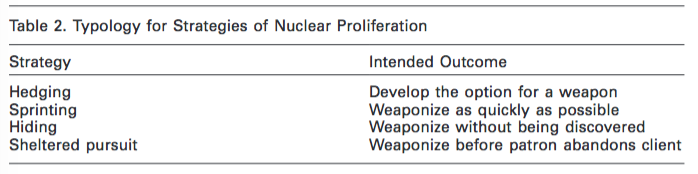
\includegraphics[width=\textwidth]{pursuitstrats.png}
    \item Look at the below flow chart it explains the model\\
    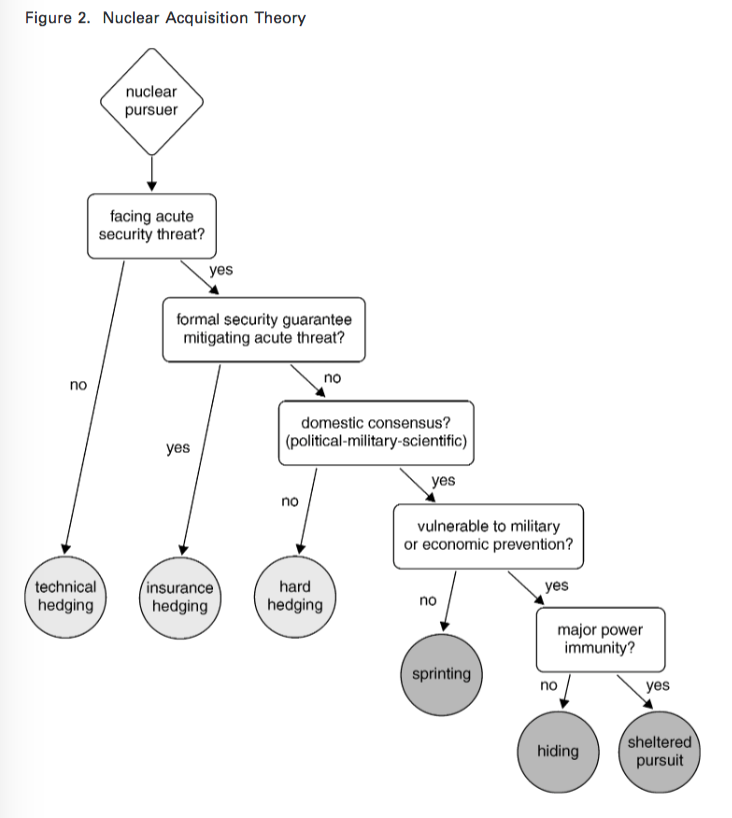
\includegraphics[width=\textwidth]{narangmodel.png}
    \item three sets of variables that states must consider
    \begin{enumerate}
        \item immediate security environment
        \item internal domestic context
        \item international constraints/opportunities
    \end{enumerate}
    \item states that are not under immediate threat may be able to simply hedge, others must make their move
    \item states can move between the strategies (look at India), often have a final sprint
    \item empirical record of his model is pretty good
    \item countries like Japan can hard hedge in order to keep their security agreements (in this case with the US)
\end{itemize}
\textit{Important points from reading guide}
\begin{enumerate}
    \item understand why he looks at the \textit{how} aspect
    \item understand differences/goals of hedging, sprinting, hiding, sheltered pursuit
    \item don't worry about memorizing India case
\end{enumerate}
\subsection*{Cyberwar}
\textbf{Rid}: \textit{Cyber War Will Not Take Place}
\begin{itemize}
    \item argument hinges on a definition of war
    \item according to Clausewitz, there are three necessary conditions for something to be a war:
    \begin{enumerate}
        \item must have violent character - potentially or actually lethal
        \item instrumental character - has a means and an end
        \item must have a political nature - war is not an isolated act, but has a larger political purpose
    \end{enumerate}
    \item no cyber attack has ever injured/killed a person, so no war
    \item DDoS is not like a naval blockade, as there is no tactical objective and stuff
    \item cyber attacks can accompany conventional attacks, but that's not cyber war I guess
    \item note that they do not need to be violent to be effective, it just means they are not acts of war
    \item what we typically have is political crime
    \item also attacks are often unclaimed, so they can't be political
    \item cyber attacks are really acts of sabotage, espionage and subversion
    \item sabotage: deliberate attempt to weaken or destroy an economic or military system - not necessarily war because they may avoid violence and political attribution, but always are instrumental
    \item espionage: penetrating an adversarial system to extract information - typically not violent, and not necessarily instrumental
    \item subversion: undermine the authority, integrity, or constitution of an established order - different than insurgency, and does not require violence
    \item contrary to conventional wisdom, the offense defense balance has not necessarily flipped - quality matters not quantity
\end{itemize}
\medskip
\textbf{Stone}: \textit{Cyber War Will Take Place!}
\begin{itemize}
    \item well, it could
    \item old-school ideas of force and violence cannot be applied to cyber attacks
    \item war involves force, but force need not actually imply violence
    \item in old, conventional wars, you got things done with physical force
    \item look at bombing raids during WWII which killed people as collateral damage, but if this had been done with cyber attacks would it not have been an act of war?
    \item lethality can just be collateral, it need not be the key element of the force
    \item according to Rid's view, those bombing runs would be considered sabotage, not war, but clearly they were war, so the two are not mutually exclusive
    \item acts of war can also be covert
    \item if technology is a ``violence multiplier", that allows small force to become large violence
    \item Stones point: cyber attacks \textit{could} constitute acts of war, so eventually they will
\end{itemize}
\medskip
\textbf{Lindsay}: \textit{Stuxnet and the Limits of Cyber Warfare}
\begin{itemize}
    \item the Cyber Revolution thesis (offense easier than defense, weaker actors get more power, attribution problem is real) is wrong! Stuxnet shows this!
    \item most malicious activity in cyberspace is financially motivated
    \item also espionage, hacktivism
    \item cyber warfare is different - it uses computers to generate force to disrupt an opponent's infrastructure
    \item so true cyber warfare is rare, but small crimes are common
    \item idea: weaker actors can use cyber warfare to make stronger actors more vulnerable
    \item cyber defense is hard, so the thinking goes that this gives cyber offense a comparative advantage
    \item deterrence does not work because attribution is hard
    \item however, Stuxnet (the only real cyber warfare case) demonstrates just the opposite
    \item Stuxnet: attack by US and Israel (probably) on Iranian nuclear material centrifuges
    \item this attack was done by the STRONG actors (whaaat?), and required significant technical planning, large infrastructure, and a long lead up period
    \item it didn't even work that well, rip the offense dominant idea
    \item it got attributed to USA/Israel pretty easily
    \item damn its almost like Stuxnet demonstrates exactly the opposite of what the Cyber Revolution Thesis says should happen, thats weird
    \item so trivial attacks may be easy to mount, but true cyber warfare is really hard still
\end{itemize}
\textit{Important points from reading guide}
\begin{enumerate}
    \item two dimensional DEBATE: does cyberwar exist? is the Cyber Revolution thesis right?
    \item understand both Rid and Stone arguments and their DEBATE
    \item Lindsay challenges the CRT, understand the CRT and his challenges
    \item who do you find the most convincing?
    \item think about these debates in the broader context of US foreign policy
\end{enumerate}
\end{document}